\documentclass{beamer}
\usetheme{Boadilla}
\usepackage{tikz}
\usepackage{booktabs}
\usepackage{siunitx}
\usepackage{amsmath}
\usepackage{relsize}
\usepackage{caption}
\usepackage{mwe}
\usepackage{booktabs}
\usepackage{amssymb}
\usepackage{wrapfig}
\usepackage{lipsum}
\usetikzlibrary{arrows,automata}

\usepackage[utf8]{inputenc}


\title[About Beamer] %optional
{Two Example With Beamer}

\subtitle{Page 97 to 100}

\title{Two Example With Beamer}
\author{Mohammadamin Raisi\\ Student Number :970087192 \\ Unit : Tehran Shomal - Shahriar}
\date{\today}



\begin{document}

\frame{\titlepage}

\begin{frame}
\frametitle{Example 6 -  Page 97}6. Convert the following NFA to an equivalent DFA.


\textbf{Solution :}

\begin{center}

\begin{tabular}{ccc}
\toprule
\multicolumn{3}{l}{$\sum$} \\
\cmidrule(r){1-1}
 States & 0 & 1 \\
    \midrule
    ${q}_{0}$ & ${q}_{0}$ & ${q}_{0}$,${q}_{1}$ \\
    ${q}_{1}$ & ${q}_{2}$ & ${q}_{2}$ \\
    ${q}_{0}$ & - & ${q}_{1}$ \\

    \bottomrule


\end{tabular}

\end{center}



\end{frame}

\begin{frame}

($[{q}_{0}]$ is the initial state and $[{q}_{1}]$ is the final state)\\
\textbf{Solution:} Conversion is done in the following ways:
\\

\begin{center}

\begin{tabular}{ccc}
\toprule
\multicolumn{3}{l}{$\sum$} \\
\cmidrule(r){1-1}
 States & 0 & 1 \\
    \midrule
    $[{q}_{0}]$ & $[{q}_{0}]$ & $[{q}_{0}$,${q}_{1}]$ \\
    $[{q}_{0}$,${q}_{1}]$ & $[{q}_{0}$,${q}_{2}]$ & $[{q}_{0}$,${q}_{1}$,${q}_{2}]$ \\
    $[{q}_{0}$,${q}_{1}$,${q}_{2}]$ & $[{q}_{0}$,${q}_{2}]$ & $[{q}_{0}$,${q}_{1}$,${q}_{2}]$ \\
    $[{q}_{0}$,${q}_{2}]$ & $[{q}_{0}]$ & $[{q}_{0}$,${q}_{1}$,${q}_{2}]$ \\

    \bottomrule


\end{tabular}

\end{center}


\end{frame}

\begin{frame}


Rename $[{q}_{0}]$ as A, $[{q}_{0}$,${q}_{1 }]$ as B, $[{q}_{0}$,${q}_{1}$,${q}_{2}]$ as C, and $[{q}_{0}$,${q}_{2}]$ as D. The beginning state is A, and
final states are B and C.

\begin{center}

\begin{tabular}{ccc}
\toprule
\multicolumn{3}{l}{$\sum$} \\
\cmidrule(r){1-1}
 States & 0 & 1 \\
    \midrule
    A & A & B \\
    B & D & C \\
    C & D & C \\
    D & A & C \\

    \bottomrule


\end{tabular}

\end{center}


\end{frame}



\begin{frame}
\frametitle{Example 9 -  Page 99}
8. Construct a DFA equivalent to the following NDFA given in the following figure.
[UPTU 2004]



\begin{center}

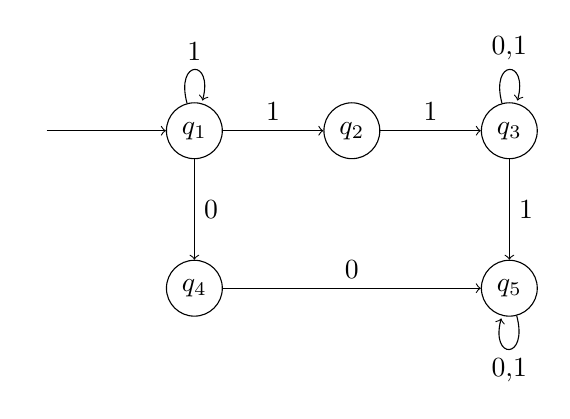
\begin{tikzpicture}[->,main/.style = {draw,circle},node distance = 2cm , auto]

\node[main] (1) {$q_1$};
\node[main] (2) [right of=1] {$q_2$};
\node[main] (3) [right of=2] {$q_3$};
\node[main] (4) [below of=1] {$q_4$};
\node[main] (5) [below of=3] {$q_5$};
\node (6) [left of=1] {};


\path (1) edge node {1} (2);
\path (2) edge node {1} (3);
\path (3) edge node {1} (5);
\path (4) edge node {0} (5);
\path (6) edge node {} (1);
\path (1) edge node {0} (4);



\path (1) edge [loop above] node {1} (1);
\path (3) edge [loop above] node {0,1}(3);
\path (5) edge [loop below] node {0,1}(5);


\end{tikzpicture}

\end{center}

\end{frame}

\begin{frame}

\textbf{Solution:} The tabular representation of the NDFA is

\begin{center}

\begin{tabular}{ccc}
\toprule
\multicolumn{2}{r}{Next State} \\
\cmidrule(r){2-3}
 Present State & 0 & 1 \\
    \midrule
    ${q}_{0}$ & ${q}_{3}$ & $\{{q}_{0}$,${q}_{1}\}$ \\
    ${q}_{1}$ & $\emptyset$ & ${q}_{2}$\\
    ${q}_{2}$& ${q}_{2}$ & $\{{q}_{2}$,${q}_{4}\}$ \\
    ${q}_{3}$ & ${q}_{4}$ & $\emptyset$ \\
    ${q}_{4}$& ${q}_{4}$ & ${q}_{4}$\\

    \bottomrule


\end{tabular}

\end{center}


\end{frame}

\begin{frame}

(${q}_{0}$ is the initial state and ${q}_{4}$ is the final state)\\
The corresponding DFA is

\begin{center}

\begin{tabular}{ccc}


\toprule
\multicolumn{3}{l}{$\sum$} \\
\cmidrule(r){1-1}
 States & 0 & 1 \\
    \midrule
    $\{{q}_{0}\}$ & $\{{q}_{3}\}$ & $\{{q}_{0}$,${q}_{1}\}$ \\
    $\{{q}_{3}\}$ & $\{{q}_{4}\}$ & $\{\emptyset\}$\\
    $\{{q}_{4}\}$& $\{{q}_{4}\}$ & $\{{q}_{4}\}$ \\
    $\{{q}_{0}$,${q}_{1}\}$ & $\{{q}_{2}\}$ & $\{{q}_{2}$,${q}_{4}\}$ \\
    $\{{q}_{2}\}$ & $\{{q}_{2}\}$ & $\{{q}_{2}$,${q}_{4}\}$ \\
    $\{{q}_{2}$,${q}_{4}\}$ & $\{{q}_{2}$,${q}_{4}\}$ & $\{{q}_{2}$,${q}_{4}\}$ \\
    $\{\emptyset\}$ & $\{\emptyset\}$ & $\{\emptyset\}$\\
    \bottomrule


\end{tabular}

\end{center}

Here $\{{q}_{0}\}$ is the beginning state, and $\{{q}_{4}\}$, and $\{{q}_{0}$,${q}_{1}\}$ are the final states.\\
(Draw a transitional diagram to complete the answer.)\\

\end{frame}
\end{document}


